\documentclass[12pt,a4paper]{article}
\usepackage[hyperref]{acl2017}
\usepackage{times}
\usepackage{latexsym}
\usepackage{graphicx}
\usepackage{url}
\usepackage{multirow}
\usepackage{tabularx}
\usepackage{graphicx}
\usepackage{tikz}
\aclfinalcopy % Uncomment this line for the final submission
%\def\aclpaperid{***} %  Enter the acl Paper ID here

%\setlength\titlebox{5cm}
% You can expand the titlebox if you need extra space
% to show all the authors. Please do not make the titlebox
% smaller than 5cm (the original size); we will check this
% in the camera-ready version and ask you to change it back.

\newcommand\BibTeX{B{\sc ib}\TeX}

\title{Temporal taggings of Entities in Text }
 
 \author{Haozhou Pang \\
  Department of Computing Science \\
  University of Alberta\\
  {\tt haozhou@ualberta.ca} \\\And
 Yourui Guo\\
  Department of Computing Science \\
  University of Alberta\\
  {\tt yourui@ualberta.ca} \\}
\date{}

\begin{document}
\maketitle

\begin{abstract}
The problem addressed in this paper aims at searching for temporal taggings that are significant to entities mentioned in articles. This task mainly consists of three phases: first, name entity recognition, which seeks phrases or strings that refer to named entities like organizations, person name and places and so on. Second, temporal expression detection, which is the process of looking for expressions in text that refers to time points or time intervals. Third, the mapping from entities to temporal expressions. In this project, we proposed a model that utilizes the lexical and syntactical information in text to tackle the problem of temporal tagging.

\end{abstract}


\section{Introduction}
 
Entities in text can be related to some time points or intervals mentioned in an article, and the demand of knowing temporal expressions that are significant to entities in articles is increasing over the years. For example, utilizing the temporal expressions can help us to look for the named entity it truly refers to. When we read a newspaper about Bush, we can interpret the named entity as George W. Bush knowing his birthdate being July 6, 1946 mentioned in the article. Also, extracting temporal expressions related to entities helps us to construct knowledge bases. As we know that most of knowledge bases contain a small quantity of temporal taggings for named entities. Thus, the content of existing knowledge bases can be expanded by providing temporal information that was taken from any source of text.

Temporal tagging detection is the process of looking for expressions in text that refers to time points or time intervals. Few works have studied on detecting temporal taggings \cite{SuTime}, \cite{HeidelTime}. SUTime \cite{SuTime} is a library for recognizing and normalizing time expressions. It transforms time expressions like “October 1963” to the normalized value of “1963-10” and type of “DATE”. Normalizing temporal expressions reduces the chance of mis-recognizing the same date value to different ones, and the result of detecting the pairs of entity and temporal tagging can be more accurate as well.

Named entities recognition seeks phrases or strings that refer to named entities like organizations, person name and places and so on. Natural Language ToolKit (NLTK) \cite{nltk} is a platform that provides us with interfaces to work with human natural language data. NLTK is utilized for natural language processing such as named entity recognition. The basic idea of recognizing named entities is to consider the task as a noun-phrase chunking. Raw text will be split into sentences first, and each sentences will be chunked by word tokenizer. Then, next step is to seeking noun phrases among chunks by tagging each chunk with pos-tagger. The last step is to use relation detection to search for potential related entities to ensure the detected entity is meaningful.

The problem addressed in this paper aims at searching for temporal taggings that are significant to entities mentioned in articles. The input can be a corpus containing multiple raw texts such as news articles, web data and social media. The output is a list of pairs that consist of both entities and temporal taggings where for each pair the entity is highly related to the temporal tagging. In this work, we need to find out all temporal taggings mentioned in plain text, and also look for entities related to them. Then, we should sort out the list of result by ranking the relatedness of entity and temporal tagging in each pair among all the pairs, and retrieve top k result with highest relatedness.

\begin{figure}
    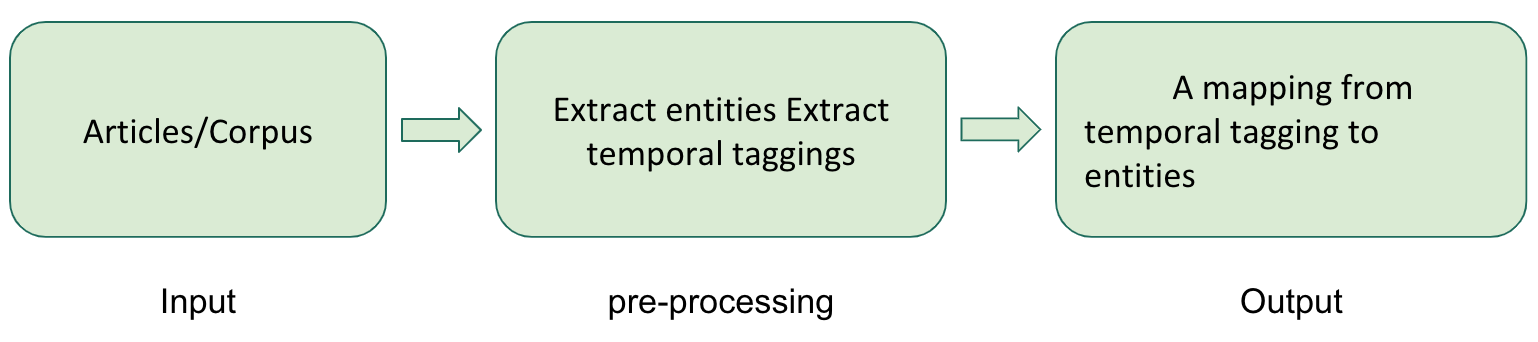
\includegraphics[width=\linewidth]{demo}
    \caption{The visualization of the process}
\end{figure}

As shown in figure.1, our task could be formulated in such way: given a set of articles with entities and meaningful temporal expressions, since we are dealing with raw text data of any format and any length, we first use the nltk sentence tokenizer \cite{nltk} to split the text into sentences, then we pre-process the sentences by extracting the candidate entities and temporal expressions, we calculate the importance score by using a series of features for each pair of entity and temporal expression so that the output will be a list of ranked pairs. The importance score is measured by adding syntactic feature and lexical feature. In this way, we can extract the most important temporal information along with their corresponding entities from a article (plain text) without assistance of any external resources.

The remainder of the paper is organized as follows: Section 2 describes the related work that addresses the same problem using other methods. Section 3 introduces the dataset and methodologies used for detecting and ranking important pairs of entity and temporal tagging,. Section 4 describes the experiments and reports the results and analysis about out experiments. Finally comes the summary and conclusion about our contributions as well as directions for future work.

\section{Related Work}
There are some papers that studied on this problem, and the concept of knowledge base is addressed to solve it where individual entities and relationships among them are stored in a large repository. Knowledge base is widely used to store complex structured and unstructured information, and knowledge bases like YAGO \cite{yago}, DBPedia \cite{dbpedia} and freebase \cite{freebase} are popular and public. The format of relation stored in knowledge base is a Subject-Predicate-Object (SPO) triple. Having the property that Knowledge base provides entities along with important facts about entities and other important temporal information,  \cite{Kuzey} proposed a method to detect temponyms and map a temporal tagging into a fact or event if present in knowledge base.

The entire process of detecting temponyms is divided into two parts. The first step is to extract important phrases from the free-text input and detect temponyms from extracted phrases. The second step is to disambiguate temponyms onto events stored in Knowledge base. Temponyms extracted from above methods consist of a large set of candidate entities. To prune candidates with low possibility of being mapped into events, mention-entity Dictionary is introduced to rank them. Top-k candidates are selected and a set of facts from Yago2 is selected if it contains the entity mentioned in top-k candidates. Some measures are applied to describe the relatedness for the mapping between temponym and facts. 

However, the method that we proposed in this paper does not build on the same ideas proposed in this paper. Knowledge base like DBPedia has a small number of temporal taggings for each entity, but there might be many time points or intervals detected in raw text that we cannot retrieve from knowledge base. So, many of results extracted from plain text will be lost as the knowledge base lacks of temporal information.

\cite{deepdive} proposed the system of Deep Dive to construct knowledge base. Unlike the construction of DBPedia \cite{dbpedia} who extracts structured content from Wikipedia, Deep Dive makes the advantage of applying Natural Language Processing (NLP) to extract useful linguistic features from plain text. Deep Dive also performs web-scale statistical learning and inferences using data-management and optimization tools.

The basic working process of Deep Dive is to first extract useful relational features from input text, and then train the statistical model that presents the correlations between linguistic patterns and target relations with those extracted features. It then uses markov logic program to combine both statistical model and additional knowledge and transform relational features to relationships of entities. In this paper, both lexical and syntactic features are used to train statistical relation-extraction model. Lexical and syntactic features are both introduced in detail in the work proposed by Mintz et al. \cite{Mintz}, and we will also present both of them that we applied in this paper in section 3.
\section{Method}
The section presents information about how we approached the current task with more detailed description about the data set. 

\subsection{Data}
Our dataset was constructed based on DBpedia dataset (version 2015-4). More specifically, we use the Extended Abstracts and Mapping-based Properties sections from DBPedia dataset.  Extended Abstracts are used as the raw text input corpus, where the selected extended abstracts contain at least one temporal expressions. Mapping-based Properties are knowledge base that store relations among entities where the data is in the format of RDF. It provides important information of entities, and helps to construct the corpus that contains the most of useful temporal expressions needed for experiments.

We designed two test set for different purpose, the first dataset was constructed by extracting all the sentences that mention about “$Barack Obama$”. This dataset contains 17148 sentences and 3491157 word tokens. The purpose of this dataset is to test whether our model can deal with the situation where one entity is related to multiple temporal expressions, and the experiment objective is to see how the different models rank the pairs differently.

The second dataset was constructed by extracting all the sentences that mention any one of the following name: $Donald$ $Trump$, $Bill$ $Clinton$, $Ronald$ $Reagan$, or $Richard$ $Nixon$. This dataset is more complicated since it contains far more name entities and meaningful temporal expressions. Also, the number of sentences / word tokens in the dataset are more than twice in the first dataset. The objective is to test whether our model can deal with larger corpus and more complex relations between entities and temporal expressions. 

The detailed statistics of the datasets are summarized in table 1.

\begin{table}[h]
\resizebox{\linewidth}{!}{%
\begin{tabular}{|c|c|c|}
\hline
 & Dataset 1 & Dataset 2 \\ \hline
Num. of sentences & 17148 & 37656 \\ \hline
Num. of word tokens & 3491157 & 7184467 \\ \hline
Num. of entities & 36233  & 76318 \\ \hline
\begin{tabular}[c]{@{}c@{}}Num. of Temporal\\ exp.\end{tabular} & 17007  & 37988 \\ \hline
\end{tabular}%
}
\caption{Statistics of the datasets}
\end{table}

\subsection{Baseline Algorithm}
We first observed some articles that contains entities and meaningful temporal expressions, we find that one entity and its corresponding temporal expression are very likely to occur in the same sentences. For example, one sentence in our dataset is that: \textit{In 2008, Barack Obama became the first African American to be elected president of the United States.}, the entity \textit{Barack Obama} and the temporal expression \textit{2008} appear in the same sentence, and we find this hypothesis are very likely to hold in a well-written article. Therefore, our baseline algorithm uses this simple heuristic by assigning a score to such pair of entity and temporal expression. At the end, all the pairs will be ranked based on the frequency of the co-occurence in one sentence. 

However, the main flaws of the baseline algorithm are that: first, the baseline does not catch the situation when the name entity and temporal expression are not in the same sentence. Second, the entities extracted by nltk are noisy, since we observed that some meaningless entities (\textit{e.g D, St}) are also extracted by nltk, which results in a significant degrade of the performance since such meaningless entities will be involved in the output. In this project, we try to tackle these problems by introducing the lexical feature and syntactic feature, which will be discussed more in detail in next section. 


\subsection{Lexical Feature}
In order to solve the situation that the entity and temporal expression are not in the same sentence, we introduce our lexical feature. It is formally defined as: \newline
\[score = \sum (w / d )\]
 \newline
where w is the weight of lexical feature, and d is the distance (number of sentences) from entity to temporal expressions. For example, one sentence in the dataset is that: \textit{Barack Obama was elected over Republican John McCain and was inaugurated on January 20, 2009. Nine months later, he was named the 2009 Nobel Peace Prize laureate.} Then entity $Barack Obama$ and the temporal expression $2009$ are not in the same sentence, but if we look at the context we will know that they are actually related. In this case, by applying the lexical feature, the pair $<$Barack Obama, 2009$>$ will also receive partial weight. 	

\subsection{Syntactic Feature}	
We try to tackle the problem of meaningless entities caused by nltk by introducing the syntactic feature. After observed some sentences in the dataset, we found that the entities usually appear at the subject position of a sentence. Therefore, we use the Stanford CoreNLP sentence parser \cite{corenlp} to extract the subject of a sentence. If the subject of a sentence happens to be an entity name, then we assign extra weight to such paris that contain the particular entity. In the example discussed in previous section, the sentence: “In 2008, Barack Obama became the first African American to be elected president of the United States.”, the pair $<$Barack Obama, 2008$>$ will be assigned a extra weight, since the entity Barack Obama is also the subject of the sentence. 

Additionally, we take a sample of 10 sentences and we find that the entities appear in the 10 sentences are all proper nouns. The intuition is that the entities of a sentences are usually person names, locations, organizations, and etc. Syntactically, such entities typically have a pos-tagging of NNP (proper noun). Based on this observation, we use nltk pos-tagger \cite{nltk} to extract all the proper nouns that appear in the dataset, and we extend our syntactic feature such that we assign extra weight to the pairs that the entity is a proper noun. 

In this way, since the meaningless entities  such as D are neither proper nouns nor subjects of a sentence. Assuming the weight given to syntactic feature is appropriate, we can filter out those meaningless entities. 



\subsection{Evaluation}
The evaluation was conducted based on the top-50 results returned from each algorithm. We manually assess each result and report the precision estimated from the top-50 results.

\section{Result}
The section present the results of the current task followed by detailed error analysis.

\subsection{dataset 1}
Our baseline model works reasonably well in the first dataset, in the top 50 pairs, 18 of them are correct. Our proposed model performs even better with 39 correct pairs out of 50. 
\begin{figure}[htbp]
\begin{minipage}[t]{0.45\linewidth}
    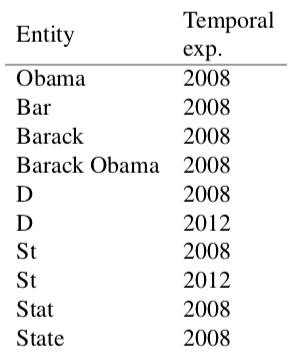
\includegraphics[width=\linewidth]{base_set1}
    \caption{baseline}
\end{minipage}%
    \hfill%
\begin{minipage}[t]{0.45\linewidth}
    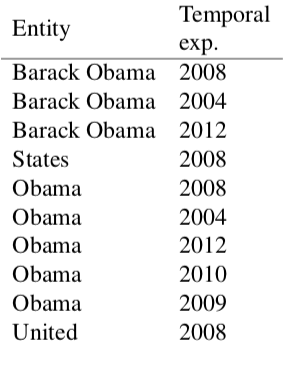
\includegraphics[width=\linewidth]{new_set1}
    \caption{our model}
\end{minipage} 
\end{figure}

Figure 2 , 3 demonstrate the top 10 results from the baseline model and our model based on dataset 1. Our model clearly extracts more meaningful pairs than the baseline.

\subsection{dataset 2}
Our Baseline model performs very poorly on this dataset, in the retrieved top 50 pairs, none of them are correct. The main issue is that the baseline model does not prune the meaningless entities, which results in all the 50 pairs contain meaningless entities. Our proposed model retrieved 13 correct pairs out of the top 50, The improvement mainly comes from the syntactic feature (entities pruning). 

\begin{figure}[htbp]
\begin{minipage}[t]{0.43\linewidth}
    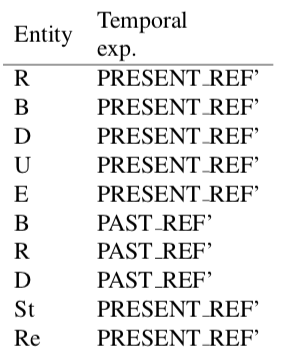
\includegraphics[width=\linewidth]{base_set2}
    \caption{baseline}
\end{minipage}%
    \hfill%
\begin{minipage}[t]{0.52\linewidth}
    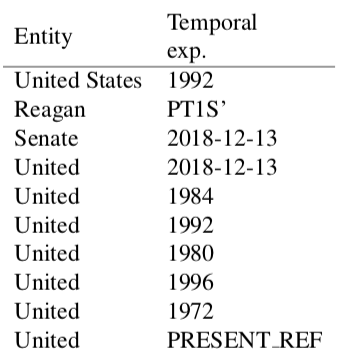
\includegraphics[width=\linewidth]{new_set2}
    \caption{our model}
\end{minipage} 
\end{figure}

As shown by Figure 4 , 5. The top 10 results from baseline is dominated by meaningless entities. After applying the lexical and syntactic features, our model can extract some correct pairs in the top 10 results.
\subsection{Error Analysis}
The most frequently captured errors could be categorized into the poor performance of nltk name entity recognizer. A great deal of the entities extracted by nltk are actually confusing. One situation happened in our experiment is that the a single English character D is considered as an entity by nltk, such entities will have high probability of co-occurrence with other temporal expressions and will be extracted by our model incorrectly, we believe our model can perform better if a better name entity recognizer is given.

\section{Conclusion}
The current task focused on investigating the relations of entities and temporal expressions in text. More specifically, we explored how to extract the important pairs of entities and temporal expressions from plain text. Given the English plain text, we used the nltk \cite{nltk} name entity recognizer to extract all the candidate entities, and we use SuTime \cite{SuTime} to extract all the candidate temporal expressions. All the pairs are ranked based on a linear combination of our lexical feature and syntactic feature. We constructed two dataset to evaluate our model, the result shows that our model performs well on the dataset with smaller size, when the dataset becomes larger and more complex, the performance of our model seems to be limited by the quality of entities extracted by nltk, but it is still significantly better than the baseline model. 
\section*{Acknowledgments}

First and far most, we would like to thank prof. Davood Rafiei for the advice and help on this project, also special thank to Michael Su for helpful discussions.

\bibliographystyle{acl_natbib}
\bibliography{ref}

\end{document}
